\documentclass[12pt]{article}
\usepackage{amsmath, amssymb, amsfonts}
\usepackage{graphicx}
\graphicspath{{Photos/}}
\usepackage{float}
\usepackage{hyperref}
\usepackage{enumitem}
\usepackage{geometry}
\usepackage{minted}
\usepackage{graphicx}
\usepackage{subcaption} 
\usepackage{booktabs}   % \toprule \midrule \bottomrule
\usepackage{siunitx}    % smart number alignment
\usepackage{array}      % column tweaks
\usepackage[margin=3cm]{geometry}

\geometry{margin=2.5cm}

\newcommand{\ddt}[1]{\frac{\partial #1}{\partial t}}
\newcommand{\ddx}[1]{\frac{\partial #1}{\partial x}}
\newcommand{\dfi}[1]{\frac{#1_{i+1} - #1_{i-1}}{2\,\Delta x}}
\newcommand{\dfii}[1]{\frac{#1_{i+1} - 2#1_i + #1_{i-1}}{\Delta x^2}}
\newcommand{\dt}[2]{\frac{u_{i}^{#2+1} - u_{i}^{#2}}{\Delta t}}


\title{Progress Report: Broyden method for nonlinear PDE}
\author{Eric Montalbán}
\date{\today}

\begin{document}
\maketitle
\tableofcontents
\newpage

\section{Introduction}
In this report, we focus on the viscous Burgers' equation and compare Newton's with Broyden's method from this nonlinear PDE.
\section{Viscous Burgers' equation}
To compare Broyden’s method and Newton’s method, we choose the viscous Burgers' equation as our candidate:
\begin{equation}
    \ddt{u} + u \ddx{u} = \nu \frac{\partial^2 u}{\partial x^2}, \quad x \in [0,1],\ t > 0
\end{equation}
with the initial condition:
\begin{equation}
    u(x,0) = \sin(\pi x)
\end{equation}
and boundary conditions:
\begin{equation}
    u(0,t) = u(1,t) = 0
\end{equation}

\section{PDE to Systems}
We begin by discretizing the nonlinear PDE, resulting in a nonlinear system. In other words, the vector $F(u^{n+1}) = 0$ cannot be written as a linear system $Au_{n+1}=b$. To solve it, we will use iterative solvers like Broyden’s, a quasi-newton method.
\\
\\
The first step is to discretize the time domain in $N_t$, $\{u^1,u^2, ... u^{N_t} \}$. Once it is done, for each time step, we will create a non-linear system of equations by discretizing the spatial domain into $N_x$ grid points and approximating spatial derivatives using central and upwind differences:

\[
\left( \frac{\partial u}{\partial x} \right)_i \approx \dfi{u}, \quad
\left( \frac{\partial^2 u}{\partial x^2} \right)_i \approx \frac{u_{i+1} - 2u_i + u_{i-1}}{\Delta x^2}
\]
To estimate the derivatives of $\ddx{u^{n+1}}$ using finite differences, there are two different kind of techniques:
\begin{itemize}
    \item Backward Euler (Implicit): It uses the same time step iterations to calculate derivates. It is naturally more accurate in detriment of the computation cost.
    \[
    \ddx{u^{n+1}}= \dfi{u^{n+1}}
    \]
    \item Forward Euler (Explicit): This one, however, is based on the known values already calculated in previous time steps iterations.We look in the past to predict the future. Therefore, it is cheaper computationally speaking but also condtiionally unstable for bigger time steps.
    \[ \ddx{u^{n+1}} = \dfi{u^{n}} 
    \]
\end{itemize}

We shall proceed by using the explicit method in nonlinear terms looking for efficiency as they are more complex than usual. For the rest of terms, we will use the traditional backward Euler method.This approach results in a semi-implicit Euler scheme. It is not Crank-Nicolson, which would involve averaging time levels; instead, we use an implicit scheme for the linear terms and an explicit scheme for the nonlinear convection.
 The result after discretizing the PDE is as follows:
\[
\dt{u}{n} + u^n \cdot \dfi{u^n} = \nu \cdot \dfii{u^{n+1}}
\]
Here we used Backward Euler (implicit) for both the time derivate and the second space derivate whereas we opted for approximating the nonlinear space derivative explicitly. This nonlinear system is then solved iteratively using either Newton's method and Broyden's method.

\section{Python: Numerical Analysis}

The nonlinear system we solve at each time step is defined by:
\[
F_i(u^{n+1})
= \dt{u}{n}
+ u_i^n\,\dfi{u^{n}}
- \nu\,\dfii{u^{n+1}}
\]


The Jacobian $J$ is a tridiagonal matrix, which using later \texttt{np.linalg.inv()}, we will be able to compute its inverse. Its entries are given by:
\[
J_{i,j}
= \frac{\partial F_i}{\partial u_j^{n+1}}
=
\begin{cases}
\displaystyle
\frac{1}{\Delta t} + \frac{2\nu}{\Delta x^2}, & j = i, \\\\[0.8em]
\displaystyle
- \frac{\nu}{\Delta x^2}, & j = i+1, \\\\[0.8em]
\displaystyle
- \frac{\nu}{\Delta x^2}, & j = i-1, \\\\[0.4em]
0, & \text{otherwise.}
\end{cases}
\]

Note that the Jacobian is of size $(N_x - 2) \\times (N_x - 2)$, as we exclude the boundary nodes due to Dirichlet conditions.


\subsection{Broyden's Method Implementation}
Broyden's method updates an approximation of the inverse Jacobian instead of recalculating it at every iteration:
We leave the algorithm as well:
\begin{figure}[H]
  \centering
  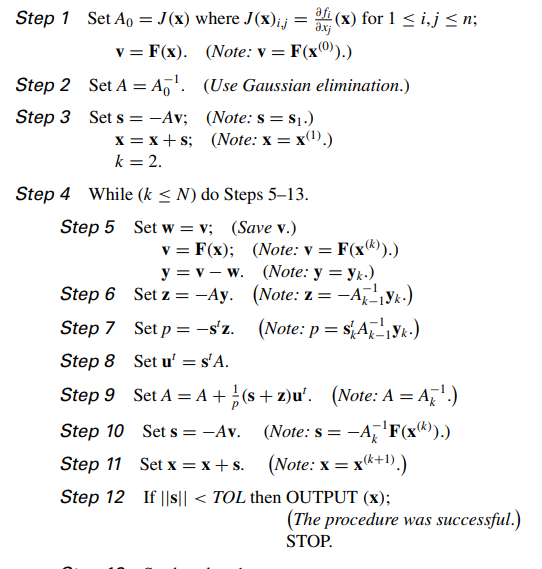
\includegraphics[width=0.7\textwidth]{image.png}
  \caption{Broyden's algorithm}
  \label{fig:burgers}
\end{figure}


\begin{minted}[linenos, breaklines]{python}
    # Parameters
L, Nx = 1, 50
T, dt = 1, 0.01
nu = 0.01
x = np.linspace(0, L, Nx)
dx = L / (Nx - 1)
Nt = int(T / dt) + 1
TOL = 1e-15
MAX_ITER = 30

# Initial condition
u0 = np.sin(np.pi * x)
u0[0] = u0[-1] = 0

def F(u, dx, dt, nu, u_old):
    f = np.zeros_like(u)
    for i in range(1, len(u) - 1):
        derivx = (u_old[i + 1] - u_old[i - 1]) / (2 * dx)
        derivxx = (u[i + 1] - 2 * u[i] + u[i - 1]) / dx**2
        f[i] = (u[i] - u_old[i]) / dt + u_old[i] * derivx - nu * derivxx
    return f

def J(u, dx, dt, nu):
    N = len(u)
    J = np.zeros((N - 2, N - 2))
    diag = 1 / dt + 2 * nu / dx**2
    sup = -nu / dx**2
    inf= sup
    for i in range(N - 2):
        if i > 0:
            J[i, i - 1] = sup
        J[i, i] = diag
        if i < N - 3:
            J[i, i + 1] = inf
    return J
def broyden(u, dx, dt, nu, TOL, N, u_old):
    Fx = F(u, dx, dt, nu, u_old)
    Jx = J(u, dx, dt, nu)
    A = np.linalg.inv(Jx)
    s = -A @ Fx[1:-1]
    u[1:-1] += s
    errors, residuals = [np.linalg.norm(s)], [np.linalg.norm(Fx)]
    
    for _ in range(1, N):
        Fx_new = F(u, dx, dt, nu, u_old)
        y = Fx_new[1:-1] - Fx[1:-1]
        z = -A @ y
        p = -s @ z
        uv = s @ A
        A += (1 / p) * np.outer(s + z, uv)
        s = -A @ Fx_new[1:-1]
        u[1:-1] += s
        errors.append(np.linalg.norm(s))
        residuals.append(np.linalg.norm(Fx_new))
        Fx = Fx_new
        if errors[-1] < TOL:
            break

    return u, errors, residuals
\end{minted}
We use the \texttt{@} operator for matrix-vector multiplication. For example, \texttt{A @ b} performs a matrix product where b is a column vector and returns a vector \texttt{c}. The function \texttt{np.outer(a, b)} computes the product of vectors \texttt{a} and \texttt{b}, resulting in a matrix that allocates in the element A(i,j) the product \texttt{a[i] * b[j]}. This is used in the rank-one update step of Broyden's method. We use \texttt{x[1:-1]} to exclude boundary conditions from updating, as they are fixed by the Dirichlet boundary condition.
\\\\
The matrix update used in Broyden’s method is based on the Sherman-Morrison formula, a rank-one update for inverse matrices:
\[
A_{k+1}^{-1} = A_k^{-1} + \frac{(s_k + z_k)(u_k)^T}{p_k}
\]

\subsection{Comparison with Newton}
Newton’s method computes the  Jacobian at each iteration, which costs \( \mathcal{O}(n^3) \) and requires \( n^2 \) functional operations.  Broyden’s method, in contrast, only needs $n$ function evaluation and updates an approximation of the inverse Jacobian, making it much cheaper. As a result, Newton offers quadratic convergence versus the superlineal convergence of Broyden but with a more friendly computational cost as we can see.
\[
\begin{array}{l|c|c|c}
\textbf{Method} & \textbf{Function Evals}  & \textbf{Jacobian Update} & \textbf{Total Cost} \\
\hline
\text{Newton} &  n^2 + n \text{ (F(u) + J(u))} & \mathcal{O}(n^3)  & \mathcal{O}(n^3) \\
\text{Broyden} & n & \mathcal{O}(n^2) \text{ (matrix*vector)} & \mathcal{O}(n^2) \\
\end{array}
\]


\subsection{Main Loop}
Broyden is called at each time step, solving $N_t$ nonlinear systems altogether.
\begin{minted}[linenos, breaklines]{python}
for n in range(1, Nt):
    u_old = u.copy()
    u = broyden(u.copy(), dx, dt, nu, TOL, N, u_old)
    U[n, :] = u
\end{minted}
\subsection{Solutions}
We got a maximum difference of 4.44e-16 when executing both methods with this parameter values: 

\begin{minted}[linenos, breaklines]{python}
# Parameters
L, Nx = 1, 100
T, dt = 0.5, 0.1
nu = 0.01
x = np.linspace(0, L, Nx)
dx = L / (Nx - 1)
Nt = int(T / dt) + 1  
TOL = 1e-15
MAX_ITER = 30
\end{minted}


\begin{figure}[H]
  \centering

  \begin{subfigure}[b]{0.6\textwidth}
    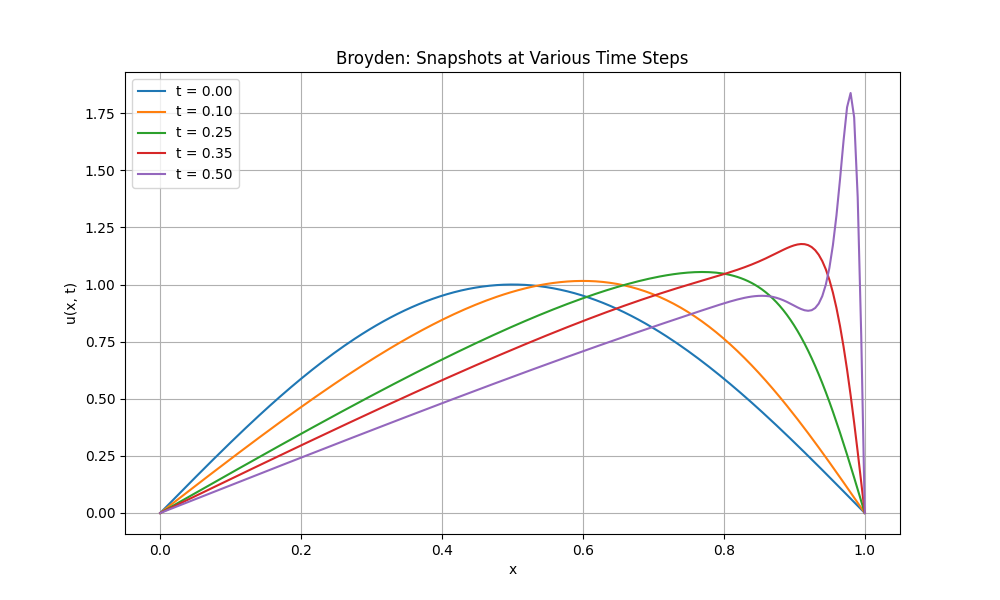
\includegraphics[width=\textwidth]{Broyden_snapshots.png}
    \caption{Broyden Snapshot}
    \label{fig:broyden_snapshot}
  \end{subfigure}
  \hfill
  \begin{subfigure}[b]{0.6\textwidth}
    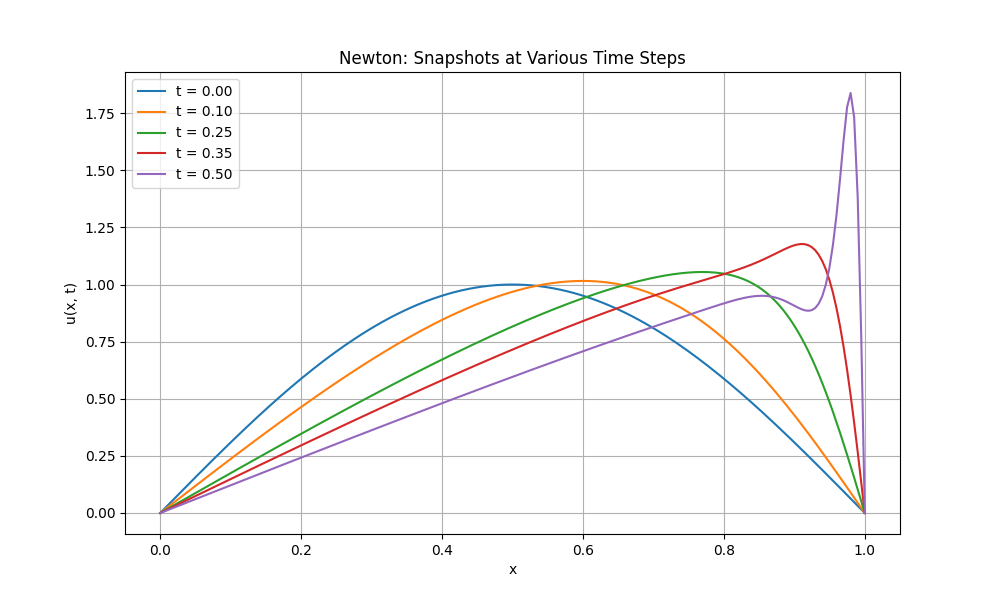
\includegraphics[width=\textwidth]{Newton_snapshots.png}
    \caption{Newton Snapshot}
    \label{fig:newton_snapshot}
  \end{subfigure}

  \vspace{0.5cm}

  \begin{subfigure}[b]{0.6\textwidth}
    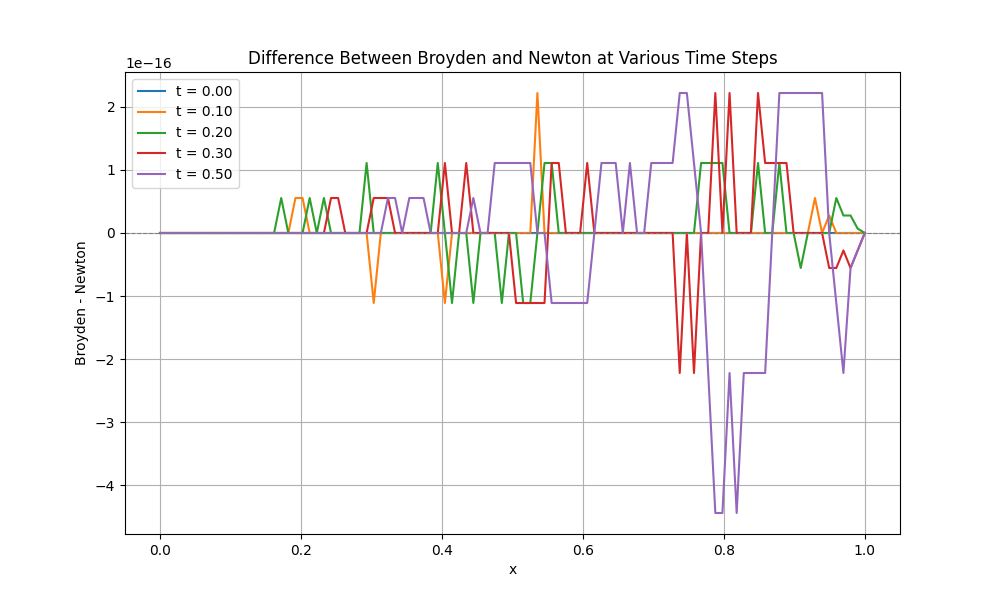
\includegraphics[width=\textwidth]{Dif_New_Broy.png}
    \caption{Difference Between Methods}
    \label{fig:difference}
  \end{subfigure}
  \hfill
  \begin{subfigure}[b]{0.6\textwidth}
    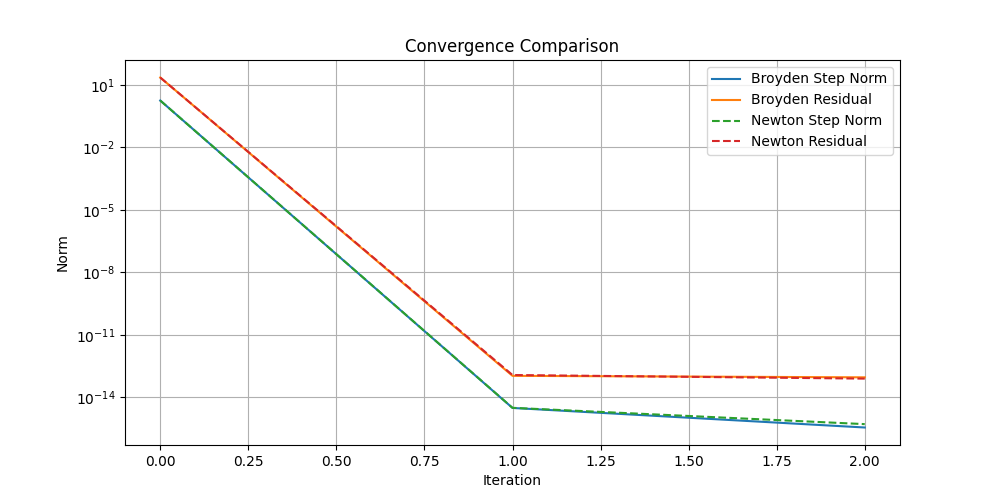
\includegraphics[width=\textwidth]{Convergence_comparison.png}
    \caption{Convergence Comparison}
    \label{fig:convergence}
  \end{subfigure}

  \caption{Comparison of Newton and Broyden Methods}
  \label{fig:four_panel}
\end{figure}


\cleardoublepage
\phantomsection
\addcontentsline{toc}{section}{References}
\begin{thebibliography}{9}

\bibitem{burden}
Burden, R. L., \& Faires, J. D. (2010). 
\textit{Numerical Analysis}. Brooks/Cole.

\bibitem{cordero2014}
Cordero, A., Soleymani, F., \& Torregrosa, J. R. (2014).  
\href{https://doi.org/10.1016/j.amc.2014.07.010}
{\textit{Dynamical analysis of iterative methods for nonlinear systems or how to deal with the dimension?}} 
Applied Mathematics and Computation.

\bibitem{kansal2020}
Kansal, M., Cordero, A., Bhalla, S., \& Torregrosa, J. R. (2020).  
\href{https://doi.org/10.1007/s11075-020-00997-4}
{\textit{New fourth- and sixth-order classes of iterative methods for solving systems of nonlinear equations and their stability analysis}}. 
Numerical Algorithms.

\bibitem{cordero2022}
Cordero, A., Garrido, N., Torregrosa, J. R., \& Triguero-Navarro, P. (2022).  
\href{https://doi.org/10.3390/sym14030442}
{\textit{Symmetry in the multidimensional dynamical analysis of iterative methods with memory}}. 
Symmetry, 14(3), 442.

\bibitem{chicharro2020}
Chicharro, F. I., Cordero, A., Garrido, N., \& Torregrosa, J. R. (2020).  
\href{https://doi.org/10.1016/j.cam.2020.113052}
{\textit{On the effect of the multidimensional weight functions on the stability of iterative processes}}. 
Journal of Computational and Applied Mathematics, 113052.

\bibitem{behl2020}
Behl, R., Cordero, A., \& Torregrosa, J. R. (2020).  
\href{https://doi.org/10.1016/j.cam.2020.113053}
{\textit{High order family of multivariate iterative methods: Convergence and stability}}. 
Journal of Computational and Applied Mathematics, 113053.

\bibitem{cordero2018}
Cordero, A., Giménez-Palacios, I., \& Torregrosa, J. R. (2019).  
\href{https://doi.org/10.1016/j.apnum.2018.12.006}
{\textit{Avoiding strange attractors in efficient parametric families of iterative methods for solving nonlinear problems}}. 
Applied Numerical Mathematics, 141, 157–172.

\end{thebibliography}

\end{document}
